\documentclass[10pt,a4paper]{report}
\usepackage[utf8]{inputenc}
\usepackage{amsfonts}
\usepackage{graphicx}
\usepackage[letterpaper, margin=1in]{geometry}
\usepackage{indentfirst}
\usepackage{tikz,pgfplots}
\usepackage{float}

\begin{document}

\title{Final: Deep NLP}
\author{Alex Shah}
\date{12/7/17}

\maketitle

\section{Strategy}

My strategy to determine which parameters to change was to research and recall the effects of each parameter on the data. For example I knew batch size would have little effect on the end results but may speed up the processing of the dataset, depending on the hardware. Since time was not of the essence to train a few epochs, I decided to focus my attention on other parameters. In this model, the only parameters which have an affect other than epochs, are the hidden units, number of recurrent steps, number of layers, and keep probability.


\begin{figure}[H]
  \begin{center}
    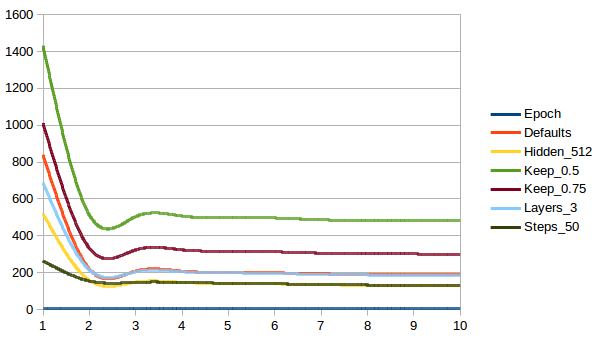
\includegraphics[width=0.75\textwidth]{epochs.png}
    \caption{Test parameters over third epoch}
  \end{center}
\end{figure}


\begin{figure}[H]
  \begin{center}
    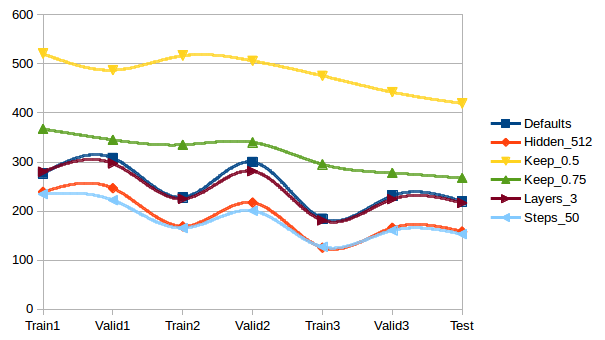
\includegraphics[width=0.75\textwidth] {train-valid-test.png}
    \caption{Training, Validation, and Test Perplexity}
  \end{center}
\end{figure}

\clearpage

\section{Most Influential Parameters}

I knew right away that some of the most influential parameters would be the number of hidden units and number of layers. Increasing these parameters would increase the overall computation space therefore increasing training time, but would most likely improve perplexity (ie decrease the value). I did not expect the best results to be from increasing the number of steps to 50. In retrospect it does make sense that increasing the number of recurrence steps would improve results. By combining the three most influential parameters the results improved even more dramatically. I also did not expect that the number of layers made nearly no difference to the training, validation, and test perplexities. The only change made by increasing the number of layers was lowering the initial perplexity which quickly fell into step with the default run.

\section{Least Influential Parameters}

Most likely this code was not optimized for changing the dropout layer. It was intially set to 1 and the results of decreasing the keep probability were adverse at worst and roughly the same at best. It would not effect results to change some of the other paramaters, other than causing vanishing/exploding gradient or other related problems. Initial weight scale would not change the results. IIncreasing the initial learning rate would make results worse until the learning rate begins to drop, and starting low would adversely affect the model. The max gradient norm just prevents against exploding gradient. Epoch related parameters involve the number of epochs at the initial training rate, then the amount of training epochs. As with any mode, more epochs would approach a better perplexity at the cost of time. Batch size, vocab size, etc, are related to processing the data and would not affect results. So the least influential of the parameters which affect perplexity was keep probability, which was only 2.

\section{Best Runs Combined}




\end{document}